\newpage
\begin{figure}[h]
	\centering
	\caption{UCA 3 - Gestione lista delle organizzazioni}
	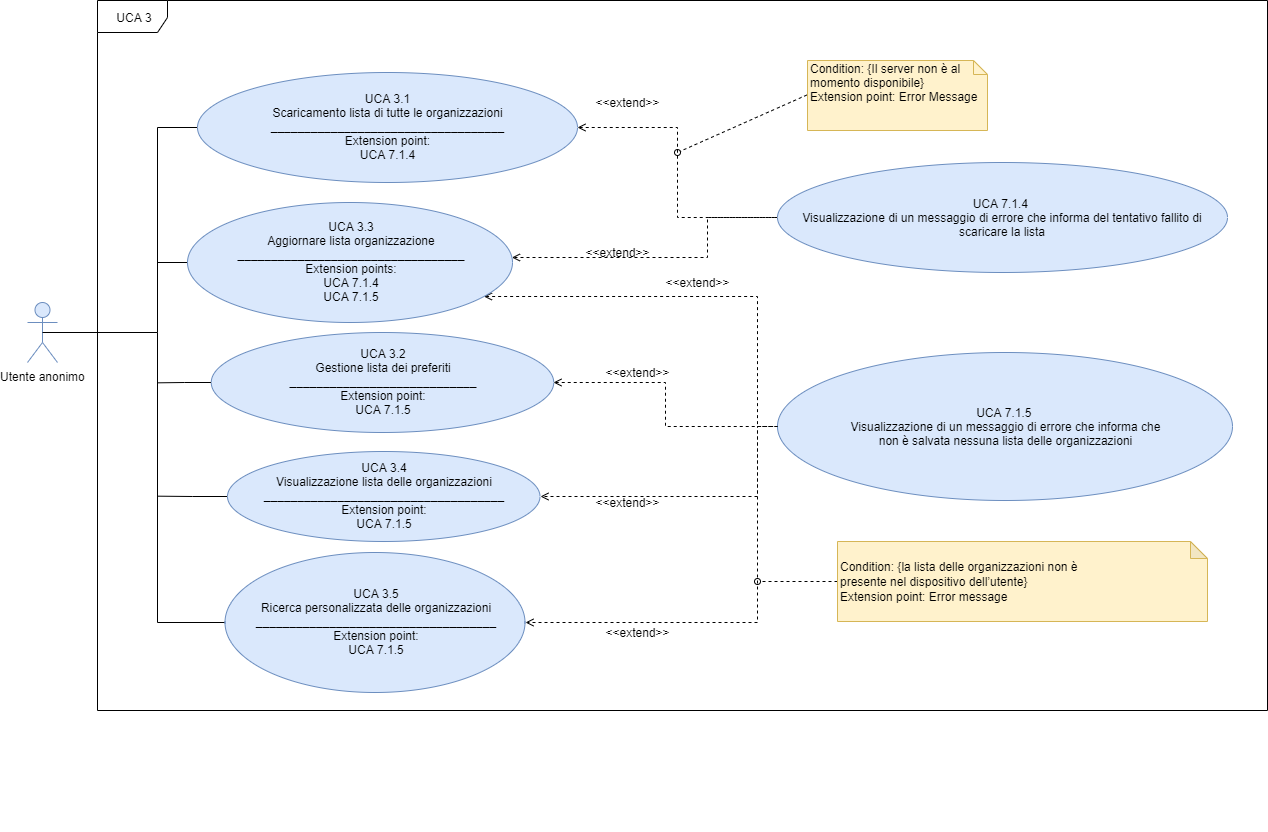
\includegraphics[scale=0.33]{sezioni/UseCase/Immagini/UCA3.png}
\end{figure}
\section{UCA 3 - Gestione lista delle organizzazioni}%kite level
\begin{itemize}
\item \textbf{Attori primari:} Utente anonimo;
\item \textbf{Attori secondari:} Server di Stalker;
\item \textbf{Precondizione:} L’utente che è stato autenticato precedentemente, esso può usufruire delle funzionalità di gestione lista delle organizzazioni;
\item \textbf{Postcondizione:} vengono forniti all’utente i risultati delle funzionalità disponibili;
\item \textbf{Scenario principale:} L’utente dell’applicazione autenticato utilizza le funzioni di gestione delle liste di organizzazioni per fare le seguenti azioni:
	\begin{itemize}
		\item Scaricare lista di tutte le organizzazioni UCA 3.1
		\item Gestione lista dei preferiti UCA 3.2
		\item Aggiornare lista di tutte le organizzazioni UCA 3.3
		\item Visualizzazione lista di tutte le organizzazioni UCA 3.4
		\item Ricerca personalizzata delle organizzazioni UCA 3.5
	\end{itemize}
\end{itemize}

\subsection{UCA 3.1 - Scaricamento lista di tutte le organizzazioni}%sea level
\begin{itemize}
\item \textbf{Attori primari:} Utente anonimo;
\item \textbf{Attori secondari: } Server di Stalker;
\item \textbf{Precondizione:} Viene reso disponibile all’utente anonimo la funzionalità di scaricare la lista di tutte le organizzazioni;
\item \textbf{Postcondizione:}Viene reso disponibile il risultato richiesto dall’utente anonimo
\item \textbf{Scenario principale:} 
\begin{itemize}
	\item L'utente selezione l'esecuzione della funzione "Scaricamento della lista";
\end{itemize}
\item \textbf{Scenario alternativo:}  Se il server stalker non è disponibile viene visualizzato all’utente un messaggio di errore che lo informa di tale problema;
\item \textbf{Estensioni:}
	\begin{enumerate}
	\item UCA 3.1.1 Visualizzazione di un messaggio di errore che informa la non disponibilità del server.
\end{enumerate}
  
\end{itemize}

\subsubsection{UCA 3.1.1 - Visualizzazione di un messaggio di errore che informa la non disponibilità del server}%fish level
\begin{itemize}
\item \textbf{Attori primari:} Utente anonimo;
\item \textbf{Precondizione:} Il Server non è attualmente disponibile;
\item \textbf{Postcondizione:} Viene visualizzato un messaggio d’errore che informa la non disponibilità del server.

\end{itemize}

\begin{figure}[h]
	\centering
	\caption{UCA 3.2 - Gestione lista dei preferiti}
	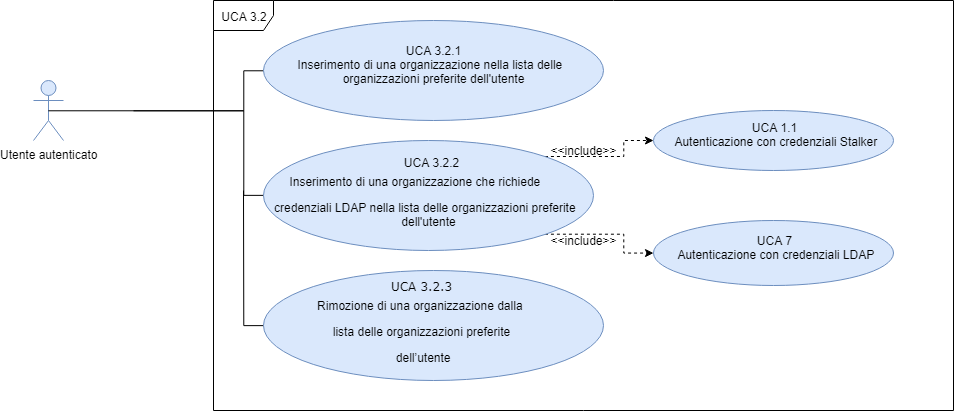
\includegraphics[scale=0.5]{sezioni/UseCase/Immagini/UCA3.2.png}
\end{figure}

\subsection{UCA 3.2 - Gestione lista dei preferiti}%sea level

\begin{itemize}
	\item \textbf{Attori primari:} Utente anonimo;
	\item \textbf{Precondizione:} Viene reso disponibile all’utente anonimo la funzionalità di gestione della lista dei preferiti; 
	\item \textbf{Postcondizione:} Viene reso disponibile il risultato richiesto dall’utente anonimo;
	\item \textbf{Scenario principale:}
			\begin{itemize}
			\item L’utente accede alla funzionalità di "Gestioni della lista dei preferiti";
			\item L'utente puo selezionare la funzione UCA 3.2.1 Inserimento di una organizzazione nella lista dei preferiti dell’utente dell’applicazione;
			\item L'utente puo selezionare la funzione UCA 3.2.2 Rimozione di una organizzazione dalla lista dei preferiti dell’utente dell’applicazione.
			\end{itemize}
	\item \textbf{Scenario alternativo:} Se non è presente nessuna lista delle organizzazioni viene visualizzato all’utente un messaggio di errore che lo informa di tale problema;
	\item \textbf{Estensioni:}
	\begin{enumerate}
		\item UCA 3.1.2 Visualizzazione di un messaggio di errore che informa che non è salvata nessuna lista delle organizzazioni.
	\end{enumerate}
\end{itemize}

\subsubsection{UCA 3.2.1 - Inserimento di una organizzazione nella lista dei preferiti dell’utente dell’applicazione}%fish level
\begin{itemize}
	\item \textbf{Attori primari:} Utente anonimo;
	\item \textbf{Precondizione:} Viene reso disponibile all’utente anonimo la funzionalità di inserimento nella lista dei preferiti; 
	\item \textbf{Postcondizione:}Viene reso disponibile il risultato richiesto dall’utente autenticato.
\end{itemize}

\subsubsection{UCA 3.2.2 - Rimozione di una organizzazione dalla lista dei preferiti dell’utente dell’applicazione}%fish level
\begin{itemize}
	\item \textbf{Attori primari:} Utente anonimo;
	\item \textbf{Precondizione:} Viene reso disponibile all’utente anonimo la funzionalità di rimozione nella lista dei preferiti;
	\item \textbf{Postcondizione:} Viene reso disponibile il risultato richiesto dall’utente autenticato.
\end{itemize}

\begin{figure}[h]
	\centering
	\caption{UCA 3.3 - Aggiornare lista organizzazione}
	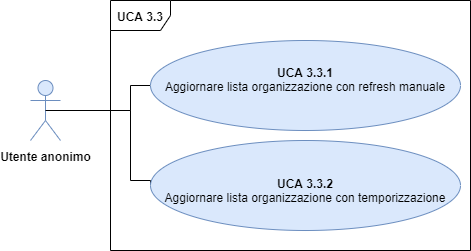
\includegraphics[scale=0.5]{sezioni/UseCase/Immagini/UCA3.3.png}
\end{figure}

\subsection{UCA 3.3 - Aggiornare lista organizzazione}%sea level
\begin{itemize} 
	\item \textbf{Attori primari:} Utente anonimo;
	\item \textbf{Attori secondari:} Server di Stalker;
	\item \textbf{Precondizione:} Viene reso disponibile all’utente anonimo la funzionalità di aggiornamento della lista di tutte le organizzazioni;
	\item \textbf{Postcondizione:} Viene reso disponibile il risultato richiesto dall’utente anonimo;
	\item \textbf{Scenario principale:}  L’utente accede alla funzione "Aggiornamento della lista" attraverso una delle due modalità disponibili
	\begin{itemize}
		\item UCA 3.3.1 Aggiornamento lista organizzazione con refresh manuale;
		\item UCA 3.3.2 Aggiornamento lista organizzazione con temporizzazione.
	\end{itemize}
	\item \textbf{Scenario alternativo:} Se il server stalker non è disponibile viene visualizzato all’utente autenticato un messaggio di errore che lo informa di tale problema;
	\item \textbf{Estensioni:}
	\begin{enumerate}
		\item UCA 3.3.3 Visualizzazione di un messaggio che informa la non disponibilità del server.
	\end{enumerate}
\end{itemize}

\subsubsection{UCA 3.3.1 - Aggiornare lista organizzazione con refresh manuale}%fish level
\begin{itemize}
	\item \textbf{Attori primari:} Utente anonimo;
	\item \textbf{Attori secondari:} Server di Stalker;
	\item \textbf{Precondizione:} Viene reso disponibile all’utente anonimo l’aggiornamento della lista dell’organizzazione attraverso la modalità refresh manuale;
	\item \textbf{Postcondizione:} Viene ottenuto il risultato richiesto dall’utente anonimo.
	
\end{itemize}

\subsubsection{UCA 3.3.2 - Aggiornare lista organizzazione con temporizzazione}%fish level
\begin{itemize} 
	\item \textbf{Attori primari:} Utente anonimo;
	\item \textbf{Attori secondari:} Server di Stalker;
	\item \textbf{Precondizione:} Viene reso disponibile all’utente anonimo l’aggiornamento della lista dell’organizzazione attraverso la modalità temporizzazione; 	
	\item \textbf{Postcondizione:} Viene ottenuto il risultato richiesto dall’utente anonimo
\end{itemize}

\subsubsection{UCA 3.3.3 - Visualizzazione di un messaggio di errore che informa che non è salvata nessuna lista delle organizzazioni}%fish level
\begin{itemize}
	\item \textbf{Attori primari:} Utente anonimo;
	\item \textbf{Precondizione:} La lista delle organizzazioni non è presente nel dispositivo dell’utente;
	\item \textbf{Postcondizione:} Viene visualizzato un messaggio di errore che informa che nel dispositivo non è presente la lista delle organizzazioni.
\end{itemize}

\newpage
\begin{figure}[h]
	\centering
	\caption{UCA 3.4 - Visualizzazione lista}
	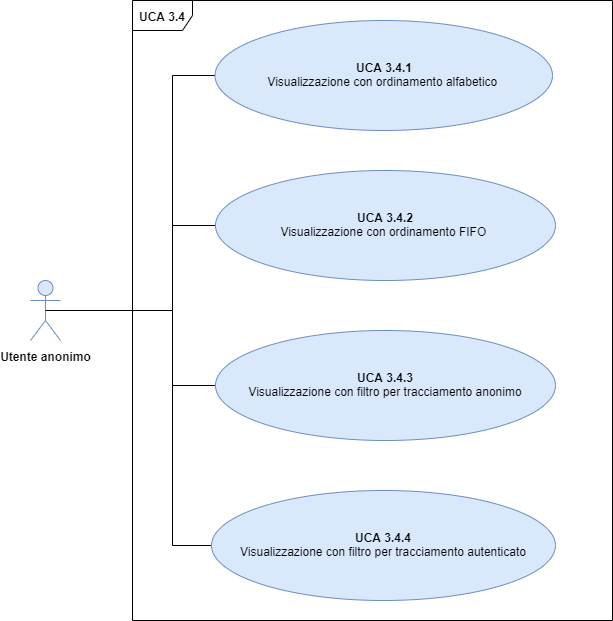
\includegraphics[scale=0.5]{sezioni/UseCase/Immagini/UCA3.4.png}
\end{figure}

\subsection{UCA 3.4 - Visualizzazione lista}%sea level

\begin{itemize} 
	\item \textbf{Attori primari:} Utente anonimo;
	\item \textbf{Precondizione:} L’utente anonimo può utilizzare la funzionalità di visualizzazione della lista;
	\item \textbf{Postcondizione:} Viene visualizzato il risultato richiesto dall’utente anonimo;
	\item \textbf{Scenario principale:}	
	\begin{itemize}
		\item L’utente esegue la funzione "Visualizzazione lista" visualizzando i nomi delle organizzazioni presenti;
		\item L'utente puo selezionare la modalità UCA 3.4.1 Ordinamento automatico (FIFO\ap{G});
		\item L'utente puo selezionare la modalità UCA 3.4.2 Ordinamento alfabetico;
		\item L'utente puo selezionare la modalità UCA 3.4.3 Filtro per tracciamento anonima;
		\item L'utente puo selezionare la modalità UCA 3.4.4 Filtro per tracciamento autenticato.
	\end{itemize}
	\item \textbf{Scenario alternativo:} Se non è presente nessuna lista delle organizzazioni viene visualizzato all’utente un messaggio di errore che lo informa di tale problema;
	\item \textbf{Estensioni:}
	\begin{enumerate}
		\item UCA 3.3.3 Visualizzazione di un messaggio di errore che informa che non è salvata nessuna lista delle organizzazioni.
	\end{enumerate}
\end{itemize}

\subsubsection{UCA 3.4.1 - Ordinamento}%fish level
\begin{itemize}
	\item \textbf{Attori primari:} Utente anonimo;
	\item \textbf{Precondizione:}L’utente anonimo può utilizzare la funzionalità di visualizzazione della lista secondo un ordinamento;
	\item \textbf{Postcondizione:} viene visualizzato il risultato richiesto dall’utente anonimo;
	\item \textbf{Specializzazione:}
	\begin{enumerate}
		\item UCA 3.4.2 Ordinamento alfabetico;
		\item UCA 3.4.3 Ordinamento automatico FIFO \ap{G}.
	\end{enumerate}
\end{itemize}

\subsubsection{UCA 3.4.2 - Ordinamento alfabetico}%fish level
\begin{itemize}
	\item \textbf{Attori primari:} Utente anonimo;
	\item \textbf{Precondizione:} l’utente anonimo può utilizzare la funzionalità di visualizzazione della lista secondo un ordinamento automatico;
	\item \textbf{Postcondizione:} viene visualizzato il risultato richiesto dall’utente.
\end{itemize}

\subsubsection{UCA 3.4.3 - Ordinamento automatico FIFO}%fish level
\begin{itemize}	
	\item \textbf{Attori primari:} Utente anonimo;
	\item \textbf{Precondizione:} L’utente autenticato può utilizzare la funzionalità di visualizzazione della lista secondo un ordinamento automatico;
	\item \textbf{Postcondizione:} Viene visualizzato il risultato richiesto dall’utente.
\end{itemize}

\subsubsection{UCA 3.4.4 - Filtro per tracciamento}%fish level
\begin{itemize}
	\item \textbf{Attori primari:} Utente anonimo;
	\item \textbf{Precondizione:} L’utente autenticato può utilizzare la funzionalità di visualizzazione della lista secondo un ordinamento automatico;
	\item \textbf{Postcondizione:} Viene visualizzato il risultato richiesto dall’utente anonimo;
	\begin{enumerate}
		\item UCA 3.4.5 Filtro per tracciamento anonimo;
		\item UCA 3.4.6 Filtro per tracciamento autenticato.
	\end{enumerate}
\end{itemize}

\subsubsection{UCA 3.4.5 - Filtro per tracciamento anonimo}%fish level
\begin{itemize}
	\item \textbf{Attori primari:} Utente anonimo;
	\item \textbf{Precondizione:} L’utente anonimo può utilizzare la funzionalità di visualizzazione della lista che permettono un tracciamento anonimo;
	\item \textbf{Postcondizione:} Viene visualizzato il risultato richiesto dall’utente anonimo.
\end{itemize}

\subsubsection{UCA 3.4.6 - Filtro per tracciamento autenticato}%fish level
\begin{itemize}
	\item \textbf{Attori primari:} Utente anonimo;
	\item \textbf{Precondizione:} L’utente anonimo può utilizzare la funzionalità di visualizzazione della lista che permettono un tracciamento autenticato;
	\item \textbf{Postcondizione:} Viene visualizzato il risultato richiesto dall’utente anonimo.
\end{itemize}

\begin{figure}[h]
	\centering
	\caption{UCA 53.5 - Ricerca personalizzata delle organizzazioni}
	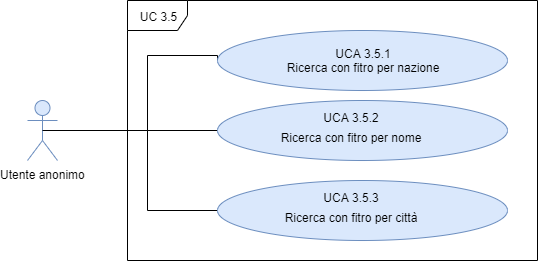
\includegraphics[scale=0.5]{sezioni/UseCase/Immagini/UCA3.5.png}
\end{figure}

\subsection{UCA 3.5 - Ricerca personalizzata delle organizzazioni}%sea level

\begin{itemize}
	\item \textbf{Attori primari:} Utente anonimo;
	\item \textbf{Precondizione:} l’utente anonimo può utilizzare la funzionalità di ricerca della lista per cercare il le organizzazioni d’interesse;
	\item \textbf{Postcondizione:} viene visualizzato il risultato richiesto dall’utente
	\item \textbf{Scenario principale:}
	\begin{itemize}
		\item L’utente anonimo accede alla funzionalità "Ricerca personalizzata" della lista delle organizzazioni per ricercare le organizzazioni a cui interessa trovare
		\item L'utente puo selezionare la modalità di ricerca UCA 3.5.1 Ricerca per nazione;
		\item L'utente puo selezionare la modalità di ricerca UCA 3.5.2 Ricerca per nome;
		\item L'utente puo selezionare la modalità di ricerca UCA 3.5.3 Ricerca per città.
	\end{itemize}
	\item \textbf{Scenario alternativo:} Se non è presente nessuna lista delle organizzazioni viene visualizzato all’utente un messaggio di errore che lo informa di tale problema;
	\item \textbf{Estensioni:}
	\begin{enumerate}
		\item UCA 3.3.3 Visualizzazione di un messaggio di errore che informa che non è salvata nessuna lista delle organizzazioni.
	\end{enumerate}
\end{itemize}

\subsubsection{UCA 3.5.1 - Ricerca per nazione}%fish level
\begin{itemize}
	\item \textbf{Attori primari:} Utente anonimo;
	\item \textbf{Precondizione:} L’utente anonimo può utilizzare la funzionalità di ricerca della lista per cercare le organizzazioni di una certa nazione d’interesse;
	\item \textbf{Postcondizione:} Viene visualizzato il risultato richiesto dall’utente anonimo.
\end{itemize}

\subsubsection{UCA 3.5.2 - Ricerca per nome}%fish level
\begin{itemize}
	\item \textbf{Attori primari:} Utente anonimo;
	\item \textbf{Precondizione:} L’utente anonimo può utilizzare la funzionalità di ricerca della lista per cercare il le organizzazioni che hanno il nome specificato dall’utente;
	\item \textbf{Postcondizione:} Viene visualizzato il risultato richiesto dall’utente anonimo.
\end{itemize}

\subsubsection{UCA 3.5.3 - Ricerca per città}%fish level
\begin{itemize}
	\item \textbf{Attori primari:} Utente anonimo;
	\item \textbf{Precondizione:} L'utente anonimo può utilizzare la funzionalità di ricerca della lista per cercare il le organizzazioni di una certa città d’interesse;
	\item \textbf{Postcondizione:} Viene visualizzato il risultato richiesto dall’utente anonimo.
\end{itemize}

